%!xelatex = 'xelatex --halt-on-error %O %S'

\documentclass{thuemp}
\begin{document}

% 标题,作者
\emptitle{}
\empauthor{王驰}{王合英}

% 奇数页页眉 % 请在这里写出第一作者以及论文题目
\fancyhead[CO]{{\footnotesize 王驰:多晶X射线衍射的物相分析及其应用}}


%%%%%%%%%%%%%%%%%%%%%%%%%%%%%%%%%%%%%%%%%%%%%%%%%%%%%%%%%%%%%%%%
% 关键词 摘要 首页脚注
%%%%%%%%关键词
\Keyword{}
\twocolumn[
\begin{@twocolumnfalse}
\maketitle

%%%%%%%%摘要
\begin{empAbstract}
\end{empAbstract}

%%%%%%%%英文标题、作者、摘要、关键词
\emptitleEn{Experiments of Modern Physics in Tsinghua University}
\empauthorEn{Chi Wang}{Heying Wang}
\KeywordEn{keyword1, keyword2, keyword3, keyword4, keyword5}

\begin{empAbstractEn}
\end{empAbstractEn}

%%%%%%%%首页角注,依次为实验时间、报告时间、学号、email
\empfirstfoot{2024-09-29}{2025-06-09}{2022012259}{chi-wang22@mails.tsinghua.edu.cn}
\end{@twocolumnfalse}
]
%%%%%%%%!首页角注可能与正文重叠,请通过调整正文中第一页的\enlargethispage{-3.3cm}位置手动校准正文底部位置:
%%%%%%%%%%%%%%%%%%%%%%%%%%%%%%%%%%%%%%%%%%%%%%%%%%%%%%%%%%%%%%%%
%  正文由此开始
\wuhao 
%  分栏开始

\section{引言}
\enlargethispage{-3.3cm}

\section{实验内容}

本实验使用X射线衍射仪,对提供的各晶体粉末样品进行X射线衍射分析,测绘出X射线衍射谱,并使用Jade 9软件对所得衍射谱进行寻峰,结合粉末衍射文件(Powder Diffraction File, PDF)卡片进行分析比对,确认物质组成,并利用Nelson-Riley外推法,对晶格常数进行精密测量。

所使用的X射线仪中【如图...】,X射线管以及探测器可相对于样品托架的法向进行对称转动,保持X射线探测方向与入射方向满足平面反射关系;在此过程中,X射线管发射出波长一定的X射线,经过托架上的样品衍射后,部分X射线进入探测器,其强度与衍射角$\theta$关系即被记录下来,形成X射线衍射谱。本实验所采用的X射线管靶材为$\text{Cu}$,使用特征谱线$\text{Cu~K\alpha}$($\lambda = 1.54059~\angstrom$)设置电压$38~\text{kV}$,电流$10~\text{mA}$,在X射线管与探测器夹角$2\theta$取$20^\circ \~ 120^\circ$的区间内,选择步长$0.03^\circ$,对样品X射线衍射谱进行测绘。

本实验所使用的样品中,已知化学组分的有多晶硅粉末($\text{Si}$)、氯化钠粉末($\text{NaCl}$)、氯化钠单晶($\text{Si}$)、铜($\text{Cu}$),钼($\text{Mo}$),石墨烯粉末($\text{C}$)、石墨粉末($\text{C}$)、金刚石粉末($\text{Si}$),另有一份白色粉末状双组分混合物A尚待本次实验测定。

\section{实验结果与分析}

\subsection{多晶硅($\text{Si}$)的X射线衍射谱测量}

\subsubsection{多晶硅晶型与X射线衍射峰分布的理论分析}

首先对多晶硅X射线衍射峰分布进行分析:在晶体衍射中,对各个晶面以及相应晶面间距$d$,其衍射峰对应衍射角$\theta$满足Bragg公式:

\begin{equation}
    2d\sin\theta  = \lambda
    \label{eq:bragg}
\end{equation}

对于晶体引入晶面常数$(h,k,l)$刻画各个取向以及间隔上的各族晶面。在硅等立方晶系晶体中,记晶格常数为$a$,可以给出相应晶面的间距$d_{hkl}$:

\begin{equation}
    d_{hkl} = \sqrt{h^2+l^2+k^2} a
    \label{eq:d_hkl}
\end{equation}

这也就对应于一系列衍射峰位置$\theta_{hkl}$:

\begin{equation}
    \sin^2 \theta_{hkl} = \frac{\lambda^2}{4a^2}(h^2+k^2+l^2)
    \label{eq:theta_hkl}
\end{equation}

晶面在衍射极大时的衍射强度与晶胞内原子位置有关,表现为受到以下结构因子调制:

\begin{equation}
    F_{hkl} = \sum_{j = 1}^{N} f_j exp{2\pi i (hx_j + ky_j + lz_j)}
    \label{eq:structure_factor}
\end{equation}

其中$f_j$为原子散射因子,$(x_j,y_j,z_j)$为原子坐标。对于硅,其具有金刚石结构(空间群:$Fd\bar{3}m$),晶胞包含8个原子(如图【】),原子分数坐标为:

\begin{align*}
(0,0,0),\quad &(0,\frac{1}{2},\frac{1}{2}),\quad (\frac{1}{2},0,\frac{1}{2}),\quad (\frac{1}{2},\frac{1}{2},0) \\
(\frac{1}{4},\frac{1}{4},\frac{1}{4}),\quad &(\frac{1}{4},\frac{3}{4},\frac{3}{4}),\quad (\frac{3}{4},\frac{1}{4},\frac{3}{4}),\quad (\frac{3}{4},\frac{3}{4},\frac{1}{4})
\end{align*}

代入计算,得到结构因子$F_{hkl}^{\text{Si}}$满足:

\begin{equation}
    |F_{hkl}^{\text{Si}}|^2 = 2|f_{\text{Si}}|^2 \cos^2 \frac{(h+k+l)\pi}{4}[1 + (-1)^{h+k} + (-1)^{h+l} + (-1)^{k+l}]^2
    \label{eq:si_struct_fac}
\end{equation}

这就给出其消光特性:

\begin{itemize}
    \item \textbf{全奇}:$h,k,l$全为奇数时,可见衍射峰;
    \item \textbf{全偶}:$h,k,l$全为偶数时,根据$(h+k+l)$分类:
        \subitem $h+k+l = 4n \quad(n\in\mathbb{Z})$:可见衍射峰;
        \subitem $h+k+l = 4n+2 \quad(n\in\mathbb{Z})$:不可见衍射峰(消光);
    \item \textbf{混合奇偶}:$h,k,l$奇偶混合时$F_{hkl}=0$(消光)。
\end{itemize}

由此可知$(111), (220), (311), (400), (331)$等晶面可观测衍射峰,而$(100), (110), (222)$等因消光不可见。这在衍射峰的分布上就表现为:

\begin{equation}
    \sin^2\theta_1 : \sin^2\theta_2: \sin^2\theta_3 : \sin^2\theta_4 : \sin^2\theta_5 : \sin^2\theta_6 : \cdots =
    3 : 8 : 11 : 16: 19: 24 \cdots
    \label{eq:si_diff_patt}
\end{equation}

\subsubsection{多晶硅X射线衍射实验数据}

在$2\theta$取$20.0^\circ \sim 120.0^\circ$范围内进行扫描,得到谱图以及Jade软件寻峰结果如下:

\begin{figure}[H]
    \centering
    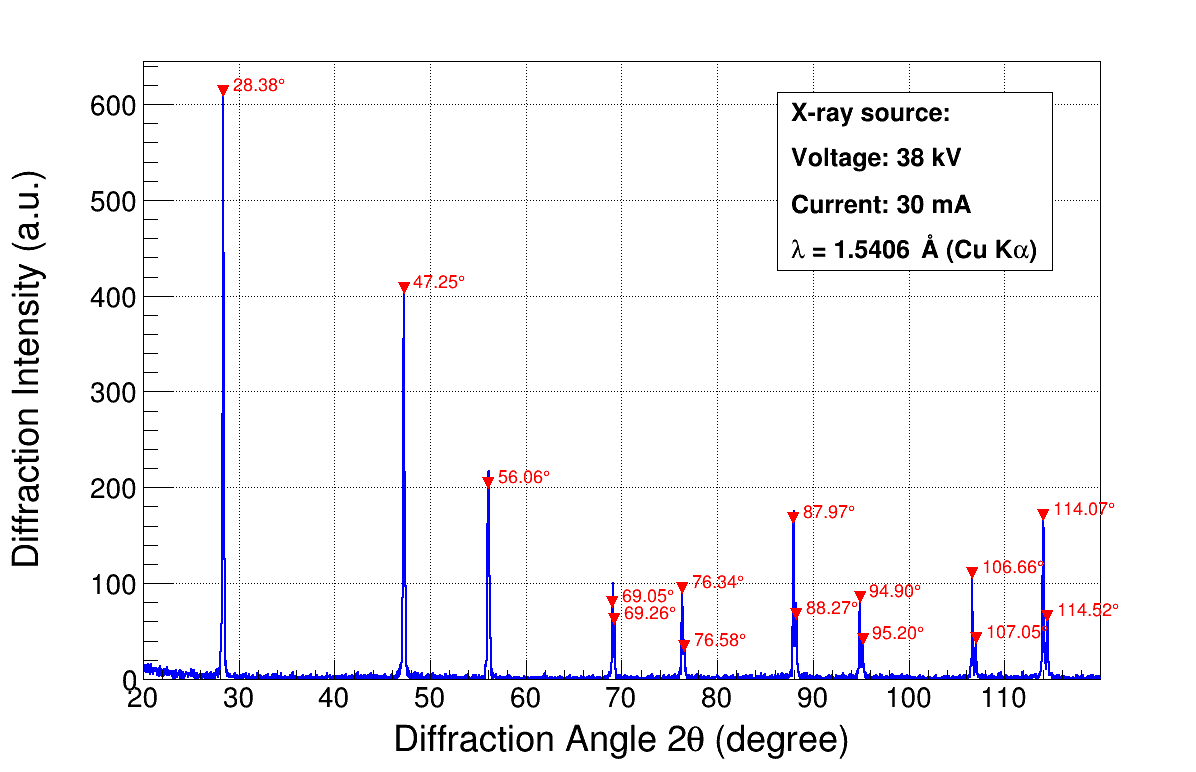
\includegraphics[options]{../Data/Silicon-multi.png}
    \caption{多晶硅粉末的X射线衍射谱图}
    \label{fig:si_xrd}    
\end{figure}

\begin{table}[H]
    \centering
    \captionnamefont{\wuhao\bf\heiti}
    \captiontitlefont{\wuhao\bf\heiti}
    \caption{多晶硅粉末X射线衍射谱寻峰结果表}
    \label{tab:si_xrd}
    \liuhao
    \begin{tabular}{ccccc}
        \toprule
        \midrule
        \bottomrule
    \end{tabular}
\end{table}

首先使用三强峰方法进行匹配以及比对:选取衍射强度最强的三个衍射峰,与PDF卡片中所载相对强度最大的衍射峰进行对比。通过Jade 9软件调取PDF#98-000-0396卡片进行对比,结果如下:

\begin{table}[H]
    \centering
    \captionnamefont{\wuhao\bf\heiti}
    \captiontitlefont{\wuhao\bf\heiti}
    \caption{多晶硅粉末X射线衍射谱三强峰法匹配结果表}
    \label{tab:si_xrd_tri_comp}
    \liuhao
    \begin{tabular}{ccccc}
        \toprule
        \midrule
        \bottomrule
    \end{tabular}
\end{table}

在以上几个衍射峰中,可以看到,衍射角度和相对强度符合得很好。进一步结合PDF卡片,标出其他衍射峰所对应晶面指数:

\begin{table}[H]
    \centering
    \captionnamefont{\wuhao\bf\heiti}
    \captiontitlefont{\wuhao\bf\heiti}
    \caption{多晶硅粉末X射线衍射峰晶面指数标定表}
    \label{tab:si_xrd_indexed}
    \liuhao
    \begin{tabular}{ccccc}
        \toprule
        \midrule
        \bottomrule
    \end{tabular}
\end{table}

所得各峰的位置与PDF卡片所载公认值符合很好,由此可以确认实验仪器以及分析方法可靠。

\subsubsection{关于多晶硅X射线“多重衍射峰”的讨论}

在本部分寻峰分析中,发现晶面指数(331)和()

\subsubsection{Nelson-Reily外推法精确测定多晶硅样品晶格常数}

在X射线衍射实验中,样品以及转动台的偏心性、样品受X射线照射样品长度有限等因素都将对衍射角$\theta$测量值引入系统误差。结合Bragg公式(式\ref{eq:bragg}),将所使用的X射线波长$\lambda$视为完全确定,可以得到不确定度关系:

\begin{equation}
    \frac{\Delta d}{d} = \cot{\theta}\Delta\theta 
    \label{eqn:d_err}
\end{equation}

由此可以推知,对于$\theta$较大区域的衍射峰,由其测量得到的晶面间距所携带的相对误差较小,因而更有利于实现精密测量。

Taylor和Sinclair于1945年更进一步地提出,以上所述及的各项系统误差,若体现在晶格常数$a$测定值中,与衍射角$\theta$的关系可以用以下函数关系描述:

\begin{equation}
    \begin{cases}
        \frac{\Delta a}{a} & \propto f(\theta) \\
        f(\theta) & = \frac{1}{2} \left(\frac{\cos^2\theta}{\sin\theta} + \frac{\cos^2\theta}{\theta}\right) \\
    \end{cases}
\end{equation}

同年,Nelson和Riley使用$\text{Cu_9Al_4}$样品进行X射线晶体衍射实验,确认这一函数可以在$\theta > 30^\circ$范围内较好描述不同吸收度样品的系统误差。实际上,考虑到$f\left(\frac{\pi}{2}\right) = 0$,可以将各个衍射峰处测得的晶格常数$a$与相应衍射角$\theta$进行$a-f(\theta)$作图,并且进行线性外推,取$\theta=\frac{\pi}{2}$时外推值,即纵轴截距$a_0$作为实际测量值。此即Nelson-Reily外推法。

对多晶硅样品,借助于Nelson-Reily外推法,有如下外推结果:

\begin{figure}[H]
    \centering
    \includegraphics[options]{../Data/Silicon-extrapolation.png}
    \caption{多晶硅样品Nelson-Riley外推法测量结果图}
    \label{fig:si_xrd_extrapol}
\end{figure}

\begin{table}[H]
    \centering
    \captionnamefont{\wuhao\bf\heiti}
    \captiontitlefont{\wuhao\bf\heiti}
    \caption{Nelson-Riley外推法测量硅晶体晶格常数数据表}
    \label{tab:si_xrd_extrapol}
    \liuhao
    \begin{tabular}{ccccc}
        \toprule
        \midrule
        \bottomrule
    \end{tabular}
\end{table}

表\ref{tab:si_xrd_extrapol}中给出的$a_0$的测量误差仅计入了外推的统计不确定度,这较于实际总不确定度仍偏小。即便如此,与PDF卡片所给参考值$a_0^{\text{Si, PDF}} = $的差值也已在不确定度范围内,进一步确认实验仪器以及分析方法可靠。

\subsection{单晶氯化钠($\text{NaCl}$)和多晶氯化钠X射线衍射谱测量}

\subsection{多晶氯化钠晶型与X射线衍射峰分布的理论分析}

多晶氯化钠的晶体结构为面心立方,晶胞包含8个原子,原子分数坐标为:

\begin{align*}
(0,0,0),\quad &(0,\frac{1}{2},0), \quad (\frac{1}{2},0,0),\quad (0,0,\frac{1}{2}) \\
(\frac{1}{2},\frac{1}{2},0),\quad &(\frac{1}{2},0,\frac{1}{2}),\quad (0,\frac{1}{2},\frac{1}{2}),\quad (\frac{1}{2},\frac{1}{2},\frac{1}{2})
\end{align*}

代入式\ref{eq:structure_factor}计算,得到结构因子:

\begin{equation}
    |F_{hkl}^{\text{NaCl}}|^2 = |\left[f_{\text{Na}}+(-1)^{h+k+l}f_\text{Cl}\right]\left[ 1 + (-1)^{h+k} + (-1)^{h+l} + (-1)^{k+l}\right]|^2
\end{equation}

这就给出其消光特性:

\begin{itemize}
    \item \textbf{全奇或全偶}:$h,k,l$全为奇数或全为偶数时,可见衍射峰;
    \item \textbf{混合奇偶}:$h,k,l$奇偶混合时$F_{hkl}=0$(消光)。
\end{itemize}

以及其衍射峰分布:

\begin{equation}
    \sin^2\theta_1 : \sin^2\theta_2: \sin^2\theta_3 : \sin^2\theta_4 : \sin^2\theta_5 : \sin^2\theta_6 : \cdots =
    3 : 4 : 8 : 11 : 12: 16 \cdots
    \label{eq:nacl_diff_patt}
\end{equation}

\subsubsection{多晶氯化钠的的X射线衍射谱测量}

使用氯化钠晶体粉末在$2\theta$取$20.0^\circ \sim 120.0^\circ$范围内进行扫描,得到谱图以及Jade软件寻峰结果如下:  

\begin{figure}[H]
    \centering
    \includegraphics[options]{../Data/NaCl-multi.png}
    \caption{多晶氯化钠粉末的X射线衍射谱图}
    \label{fig:nacl_xrd_multi}
\end{figure}

\begin{table}[H]
    \centering
    \captionnamefont{\wuhao\bf\heiti}
    \captiontitlefont{\wuhao\bf\heiti}
    \caption{多晶氯化钠粉末X射线衍射谱寻峰结果表}
    \label{tab:nacl_xrd_multi}
    \liuhao
    \begin{tabular}{ccccc}
        \toprule
        \midrule
        \bottomrule
    \end{tabular}
\end{table}

此处注意到各衍射峰极大对应衍射角$\theta$与多晶硅样品的衍射峰分布(式\ref{eq:si_diff_patt})有明显不同,且符合式\ref{eq:nacl_diff_patt},这表明多晶氯化钠样品的确为面心立方晶体结构。

此外,在峰强度方面,可以注意到无论是在PDF卡片中,还是在本实验中,“全奇”峰的强度均显著低于“全偶”峰的强度,甚而(3,3,1)晶面衍射峰在本实验中几乎不可见。这应是来自于形状因子中$(f_\text{Na} + f_\text{Cl} (-1)^{h+k+l})$一项的调制,并且由此可见,氯化钠中钠原子和氯原子的散射因子$f_\text{Na}$和$f_\text{Cl}$的大小差异不大。

\subsubsection{单晶氯化钠的的X射线衍射谱测量}

借助一金属制样品托架装夹单晶氯化钠,在$2\theta$取$20.0^\circ \sim 120.0^\circ$范围内进行扫描,得到谱图以及Jade软件寻峰结果如下:

\begin{figure}[H]
    \centering
    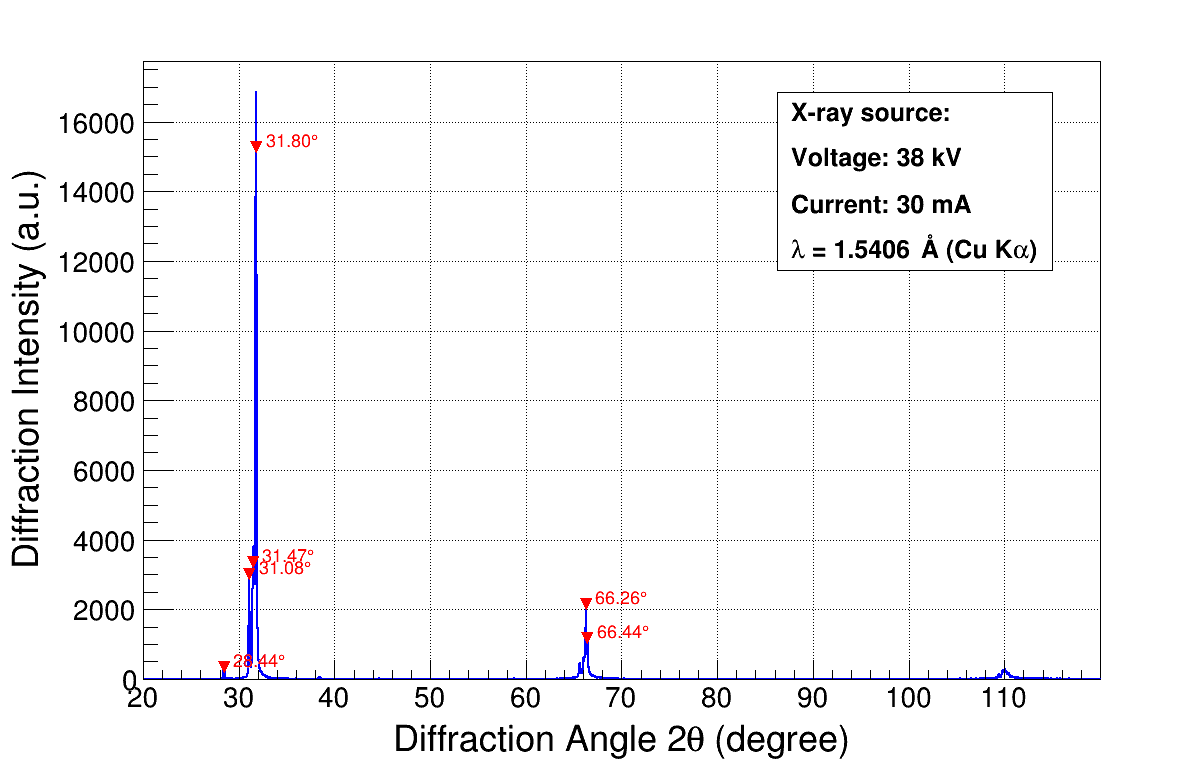
\includegraphics[options]{../Data/NaCl-single.png}
    \caption{单晶氯化钠的X射线衍射谱图}
    \label{fig:nacl_xrd_single}
\end{figure}

\begin{table}[H]
    \centering
    \captionnamefont{\wuhao\bf\heiti}
    \captiontitlefont{\wuhao\bf\heiti}
    \caption{单晶氯化钠X射线衍射谱寻峰结果表}
    \label{tab:nacl_xrd_single}
    \liuhao
    \begin{tabular}{ccccc}
        \toprule
        \midrule
        \bottomrule
    \end{tabular}
\end{table}

\subsubsection{样品托架本底的排除}

在单晶氯化钠的X射线衍射谱中,出现了一个高度显著低于其他衍射峰的衍射峰,位于$2\theta \approx 38^\circ$处。经过与氯化钠的PDF卡片初步比对,发现此处并非氯化钠的衍射峰,据此推断该衍射峰可能是样品托架的本底信号。为确证这一点,将样品托架空载进行X射线衍射测量,得到其衍射谱图以及Jade软件寻峰结果如下:

\begin{figure}[H]
    \centering
    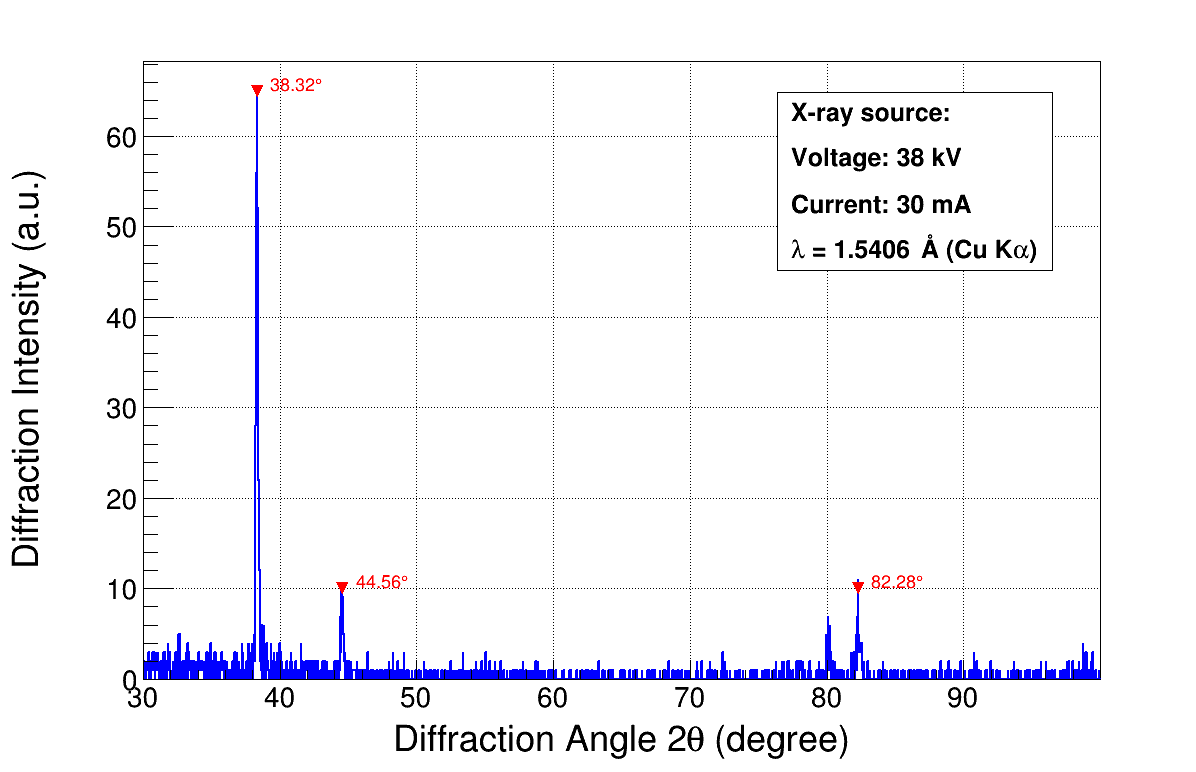
\includegraphics[options]{../Data/Background-from-manifold.png}
    \caption{样品托架空载的X射线衍射谱图}
    \label{fig:nacl_xrd_holder}
\end{figure}

\begin{table}[H]
    \centering
    \captionnamefont{\wuhao\bf\heiti}
    \captiontitlefont{\wuhao\bf\heiti}
    \caption{样品托架空载X射线衍射谱寻峰结果表}
    \label{tab:nacl_xrd_holder}
    \liuhao
    \begin{tabular}{ccccc}
        \toprule
        \midrule
        \bottomrule
    \end{tabular}
\end{table}

结合峰位置以及相对强度,可以看到,样品托架的本底信号确实在$2\theta \approx 38^\circ$处有一个显著衍射峰。由此可以确认单晶氯化钠的X射线衍射谱中该处的衍射峰确实是样品托架的本底信号。后面如未经说明,此托架的本底信号均已排除。

\subsubsection{单晶氯化钠与多晶氯化钠X射线衍射谱对比}

将单晶氯化钠的X射线衍射谱与多晶氯化钠的X射线衍射谱进行对比,我们注意到,

\subsubsection{从多晶氯化钠X射线衍射谱测定氯化晶格常数}

根据表\ref{tab:nacl_xrd_multi}当中数据进行Nelson-Riley外推,得到多晶氯化钠样品的晶格常数$a_0$的测量结果如下:

\begin{figure}[H]
    \centering
    \includegraphics[options]{../Data/NaCl-extrapolation.png}
    \caption{多晶氯化钠样品Nelson-Riley外推法测量结果图}
    \label{fig:nacl_xrd_extrapol}
\end{figure}

\begin{table}[H]
    \centering
    \captionnamefont{\wuhao\bf\heiti}
    \captiontitlefont{\wuhao\bf\heiti}
    \caption{Nelson-Riley外推法测量氯化钠晶体晶格常数数据表}
    \label{tab:nacl_xrd_extrapol}
    \liuhao
    \begin{tabular}{ccccc}
        \toprule
        \midrule
        \bottomrule
    \end{tabular}
\end{table}

所得结果与PDF卡片所给参考值$a_0^{\text{NaCl, PDF}} = 5.6402~\text{\si\angstrom}$的差值在不确定度范围内,符合较好。

\subsection{铜($\text{Cu}$)和钼($\text{Mo}$)的X射线衍射谱测量}

\subsubsection{钼的X射线衍射谱分析}

钼的晶体结构为体心立方(BCC),其晶胞包含2个原子,原子分数坐标为:

\begin{align*}
(0,0,0),\quad (\frac{1}{2},\frac{1}{2},\frac{1}{2})
\end{align*}

同样基于式\ref{eq:structure_factor},可以得到其结构因子:
\begin{equation}
    |F_{hkl}^{\text{Mo}}|^2 = 2|f_{\text{Mo}}|^2 (1+(-1)^{h+k+l})^2
    \label{eq:mo_struct_fac}
\end{equation}

得到其消光特性:

\begin{itemize}
    \item $(h+k+l)$为偶数时,可见衍射峰;
    \item $(h+k+l)$为奇数时$F_{hkl}=0$(消光)。
\end{itemize}

以及其衍射峰分布:

\begin{equation}
    \sin^2\theta_1 : \sin^2\theta_2: \sin^2\theta_3 : \sin^2\theta_4 : \sin^2\theta_5 : \sin^2\theta_6 : \cdots =
    1 : 2 : 3 : 4 : 5 : 6 \cdots
    \label{eq:mo_diff_patt}
\end{equation}
在本实验中,于$2\theta$取$20.0^\circ \sim 150^\circ$范围内进行扫描,得到谱图以及Jade软件寻峰结果如下:

\begin{figure}[H]
    \centering
    \includegraphics[options]{../Data/Molybdenum.png}
    \caption{钼的X射线衍射谱图}
    \label{fig:mo_xrd}
\end{figure}

\begin{table}
    \centering
    \captionnamefont{\wuhao\bf\heiti}
    \captiontitlefont{\wuhao\bf\heiti}
    \caption{钼X射线衍射谱寻峰结果表}
    \label{tab:mo_xrd}
    \liuhao
    \begin{tabular}{ccccc}
        \toprule
        \midrule
        \bottomrule
    \end{tabular}
\end{table}

\subsubsection{铜的X射线衍射谱分析}

铜的晶体结构为面心立方(FCC),其晶胞包含4个原子,原子分数坐标为:

\begin{align*}
(0,0,0),\quad &(0,\frac{1}{2},\frac{1}{2}),\quad (\frac{1}{2},0,\frac{1}{2}),\quad (\frac{1}{2},\frac{1}{2},0)
\end{align*}

同样基于式\ref{eq:structure_factor},可以得到其结构因子:

\begin{equation}
    |F_{hkl}^{\text{Cu}}|^2 = 4|f_{\text{Cu}}|^2[1 + (-1)^{h+k} + (-1)^{h+l} + (-1)^{k+l}]^2
    \label{eq:cu_struct_fac}
\end{equation}

其消光特性与氯化钠类似:

\begin{itemize}
    \item \textbf{全奇或全偶}:$h,k,l$全为奇数或全为偶数时,可见衍射峰;
    \item \textbf{混合奇偶}:$h,k,l$奇偶混合时$F_{hkl}=0$(消光)。
\end{itemize}

其衍射峰亦有类似于氯化钠的特点:

\begin{equation}
    \sin^2\theta_1 : \sin^2\theta_2: \sin^2\theta_3 : \sin^2\theta_4 : \sin^2\theta_5 : \sin^2\theta_6 : \cdots =
    3 : 4 : 8 : 11 : 12: 16 \cdots
    \label{eq:cu_diff_patt}
\end{equation}

在本实验中,于$2\theta$取$20.0^\circ \sim 98.3^\circ$范围内进行扫描,得到谱图以及Jade软件寻峰结果如下:

\begin{figure}[H]
    \centering
    \includegraphics[options]{../Data/Copper.png}
    \caption{铜的X射线衍射谱图}
    \label{fig:cu_xrd}
\end{figure}

\begin{table}
    \centering
    \captionnamefont{\wuhao\bf\heiti}
    \captiontitlefont{\wuhao\bf\heiti}
    \caption{铜X射线衍射谱寻峰结果表}
    \label{tab:cu_xrd}
    \liuhao
    \begin{tabular}{ccccc}
        \toprule
        \midrule
        \bottomrule
    \end{tabular}
\end{table}

寻峰结果和PDF卡片中所载的铜的衍射谱对比,发现其衍射峰位置和相对强度符合得很好。

\subsubsection{铜和钼的X射线衍射谱对比}

将铜和钼的X射线衍射谱进行对比,我们注意到,虽然两者同为立方晶系,但其衍射峰分布有明显不同,主要体现在“全奇”之外的衍射峰的消光特性上。此外值得注意的是,在铜的X射线衍射谱中,(111),(311)等“全奇”峰的强度未表现出氯化钠衍射谱中的“压低”现象,由此可更显著地看到,虽同为面心立方晶体结构,铜和氯化钠的晶体结构仍有显著差异。

\subsubsection{从铜和钼X射线衍射谱测定晶格常数}

根据表\ref{tab:cu_xrd}和表\ref{tab:mo_xrd}当中数据进行Nelson-Riley外推,得到铜和钼样品的晶格常数$a_0$的测量结果如下:

\begin{figure}[H]
    \centering
    \includegraphics[options]{../Data/Cu-extrapolation.png}
    \caption{铜样品Nelson-Riley外推法测量结果图}
    \label{fig:cu_xrd_extrapol}
\end{figure}

\begin{table}[H]
    \centering
    \captionnamefont{\wuhao\bf\heiti}
    \captiontitlefont{\wuhao\bf\heiti}
    \caption{Nelson-Riley外推法测量铜晶体晶格常数数据表}
    \label{tab:cu_xrd_extrapol}
    \liuhao
    \begin{tabular}{ccccc}
        \toprule
        \midrule
        \bottomrule
    \end{tabular}
\end{table}

\begin{figure}[H]
    \centering
    \includegraphics[options]{../Data/Mo-extrapolation.png}
    \caption{钼样品Nelson-Riley外推法测量结果图}
    \label{fig:mo_xrd_extrapol}
\end{figure}

\begin{table}[H]
    \centering
    \captionnamefont{\wuhao\bf\heiti}
    \captiontitlefont{\wuhao\bf\heiti}
    \caption{Nelson-Riley外推法测量钼晶体晶格常数数据表}
    \label{tab:mo_xrd_extrapol}
    \liuhao
    \begin{tabular}{ccccc}
        \toprule
        \midrule
        \bottomrule
    \end{tabular}
\end{table}

以上实验结果和PDF卡片给出的参考值符合均较好。

\subsection{石墨、石墨烯和金刚石的X射线衍射谱测量}

\subsubsection{石墨的X射线衍射谱测量}

在$2\theta$取$20.0^\circ \sim 120.0^\circ$范围内进行扫描,得到谱图以及Jade软件寻峰结果如下:

\begin{figure}[H]
    \centering
    \includegraphics[options]{../Data/Graphite.png}
    \caption{石墨的X射线衍射谱图}
    \label{fig:graphite_xrd}
\end{figure}

\begin{table}
    \centering
    \captionnamefont{\wuhao\bf\heiti}
    \captiontitlefont{\wuhao\bf\heiti}
    \caption{石墨X射线衍射谱寻峰结果表}
    \label{tab:graphite_xrd}
    \liuhao
    \begin{tabular}{ccccc}
        \toprule
        \midrule
        \bottomrule
    \end{tabular}
\end{table}

可以看到石墨最主要的衍射峰位于$2\theta \approx 26.5^\circ$处,且其他峰衍射强度均较弱。这一点很明显地与前面所见的各类晶体的衍射谱不同。考虑到石墨的层状结构,其层与层之间的相对位置并不十分规整,因而其衍射谱中最主要的衍射峰仅有层内原子间距的衍射峰。除此之外,最高的的衍射峰对应的晶面指数应推断为$(【】)$,提示其层间原子间距仍较为固定。

\subsubsection{石墨烯的X射线衍射谱测量}

在$2\theta$取$20.0^\circ \sim 120.0^\circ$范围内对石墨烯粉末进行扫描,得到谱图以及Jade软件寻峰结果如下: 

\begin{figure}[H]
    \centering
    \includegraphics[options]{../Data/Graphene.png}
    \caption{石墨烯的X射线衍射谱图}
    \label{fig:graphene_xrd}
\end{figure}

\begin{table}
    \centering
    \captionnamefont{\wuhao\bf\heiti}
    \captiontitlefont{\wuhao\bf\heiti}
    \caption{石墨烯X射线衍射谱寻峰结果表}
    \label{tab:graphene_xrd}
    \liuhao
    \begin{tabular}{ccccc}
        \toprule
        \midrule
        \bottomrule
    \end{tabular}
\end{table}



\subsubsection{金刚石的X射线衍射谱测量}

在$2\theta$取$20.0^\circ \sim 120.0^\circ$范围内对金刚石粉末进行扫描,得到谱图以及Jade软件寻峰结果如下:

\begin{figure}[H]
    \centering
    \includegraphics[options]{../Data/Diamond.png}
    \caption{金刚石的X射线衍射谱图}
    \label{fig:diamond_xrd}
\end{figure}

\begin{table}
    \centering
    \captionnamefont{\wuhao\bf\heiti}
    \captiontitlefont{\wuhao\bf\heiti}
    \caption{金刚石X射线衍射谱寻峰结果表}
    \label{tab:diamond_xrd}
    \liuhao
    \begin{tabular}{ccccc}
        \toprule
        \midrule
        \bottomrule
    \end{tabular}
\end{table}

可以见到,金刚石的X射线衍射谱和硅的X射线衍射谱有很大的相似性,且其衍射峰分布模式与硅的衍射峰分布模式(式\ref{eq:si_diff_patt})相同。

\subsubsection{石墨、石墨烯和金刚石的X射线衍射谱对比}



\subsection{对一组分未知的混合物A进行定性物相分析}

\subsubsection{混合物A的X射线衍射谱测量}

在$2\theta$取$20.0^\circ \sim 120.0^\circ$范围内对混合物A进行扫描,得到谱图以及Jade软件寻峰结果如下:

\begin{figure}[H]
    \centering
    \includegraphics[options]{../Data/Mixture-A.png}
    \caption{混合物A的X射线衍射谱图}
    \label{fig:mixture_a_xrd}
\end{figure}

\begin{table}
    \centering
    \captionnamefont{\wuhao\bf\heiti}
    \captiontitlefont{\wuhao\bf\heiti}
    \caption{混合物A的X射线衍射谱寻峰结果表}
    \label{tab:mixture_a_xrd}
    \liuhao
    \begin{tabular}{ccccc}
        \toprule
        \midrule
        \bottomrule
    \end{tabular}
\end{table}

\subsubsection{混合物A组分分析}

注意到混合物A的衍射峰中,有一组与此前观察过的氯化钠的衍射峰位置以及相对强度均非常接近:

\begin{table}p[H]
    \centering
    \captionnamefont{\wuhao\bf\heiti}
    \captiontitlefont{\wuhao\bf\heiti}
    \caption{混合物A与氯化钠衍射峰位置对照表}
    \label{tab:mixture_a_nacl_peaks}
    \liuhao
    \begin{tabular}{ccccc}
        \toprule
        \midrule
        \bottomrule
    \end{tabular}
\end{table}

由此可以推测,混合物A中很可能含有氯化钠。

进一步考察余下的衍射峰位置以及相对强度,观察到其衍射峰分布模式:

\begin{equation}
    \sin{\theta_1} : \sin{\theta_2} :\sin{\theta_3} : \sin{\theta_4} : \cdots = 1 : 2 : 3 : 4 : \cdots
    \label{eq:mixture_a_diff_patt}
\end{equation}

这符合【】晶型的X射线衍射谱特征。对此进一步进行标定:

结合消光特性以及测得的晶格常数,查阅PDF卡片,判断混合物A中可能含有【】晶型的【】。

更进一步地对比:

\begin{table}[H]
    \centering
    \captionnamefont{\wuhao\bf\heiti}
    \captiontitlefont{\wuhao\bf\heiti}
    \caption{混合物A与氯化钠以及【】衍射峰位置对照表}
    \label{tab:mixture_a_unknow_peaks}
    \liuhao
    \begin{tabular}{ccccc}
        \toprule
        \midrule
        \bottomrule
    \end{tabular}
\end{table}

至此,混合物A的各个衍射峰均已有对应的物相,且与PDF卡片中所载的各物相的衍射谱符合得很好,可判断混合物A主要组分为氯化钠和【】。

\section{结论}


%%%%%%%%%%%%%%%%%%%%%%%%%%%%%%%%%%%%%%%%%%%%%%%%%%%%%%%%%%%%%%%%
%  参考文献
%%%%%%%%%%%%%%%%%%%%%%%%%%%%%%%%%%%%%%%%%%%%%%%%%%%%%%%%%%%%%%%%
%  参考文献按GB/T 7714-2015《文后参考文献著录规则》的要求著录. 
%  参考文献在正文中的引用方法:\cite{bib文件条目的第一行}

\renewcommand\refname{\heiti\wuhao\centerline{参考文献}\global\def\refname{参考文献}}
\vskip 12pt


\let\OLDthebibliography\thebibliography
\renewcommand\thebibliography[1]{
  \OLDthebibliography{#1}
  \setlength{\parskip}{0pt}
  \setlength{\itemsep}{0pt plus 0.3ex}
}

{
\renewcommand{\baselinestretch}{0.9}
\liuhao
\bibliographystyle{gbt7714-numerical}
\bibliography{./Report/TempExample}
}

\appendix
\section{衍射谱寻峰数据}


\end{document}
